% Options for packages loaded elsewhere
\PassOptionsToPackage{unicode}{hyperref}
\PassOptionsToPackage{hyphens}{url}
%
\documentclass[
]{article}
\usepackage{amsmath,amssymb}
\usepackage{lmodern}
\usepackage{iftex}
\ifPDFTeX
  \usepackage[T1]{fontenc}
  \usepackage[utf8]{inputenc}
  \usepackage{textcomp} % provide euro and other symbols
\else % if luatex or xetex
  \usepackage{unicode-math}
  \defaultfontfeatures{Scale=MatchLowercase}
  \defaultfontfeatures[\rmfamily]{Ligatures=TeX,Scale=1}
\fi
% Use upquote if available, for straight quotes in verbatim environments
\IfFileExists{upquote.sty}{\usepackage{upquote}}{}
\IfFileExists{microtype.sty}{% use microtype if available
  \usepackage[]{microtype}
  \UseMicrotypeSet[protrusion]{basicmath} % disable protrusion for tt fonts
}{}
\makeatletter
\@ifundefined{KOMAClassName}{% if non-KOMA class
  \IfFileExists{parskip.sty}{%
    \usepackage{parskip}
  }{% else
    \setlength{\parindent}{0pt}
    \setlength{\parskip}{6pt plus 2pt minus 1pt}}
}{% if KOMA class
  \KOMAoptions{parskip=half}}
\makeatother
\usepackage{xcolor}
\usepackage[margin=1in]{geometry}
\usepackage{color}
\usepackage{fancyvrb}
\newcommand{\VerbBar}{|}
\newcommand{\VERB}{\Verb[commandchars=\\\{\}]}
\DefineVerbatimEnvironment{Highlighting}{Verbatim}{commandchars=\\\{\}}
% Add ',fontsize=\small' for more characters per line
\usepackage{framed}
\definecolor{shadecolor}{RGB}{248,248,248}
\newenvironment{Shaded}{\begin{snugshade}}{\end{snugshade}}
\newcommand{\AlertTok}[1]{\textcolor[rgb]{0.94,0.16,0.16}{#1}}
\newcommand{\AnnotationTok}[1]{\textcolor[rgb]{0.56,0.35,0.01}{\textbf{\textit{#1}}}}
\newcommand{\AttributeTok}[1]{\textcolor[rgb]{0.77,0.63,0.00}{#1}}
\newcommand{\BaseNTok}[1]{\textcolor[rgb]{0.00,0.00,0.81}{#1}}
\newcommand{\BuiltInTok}[1]{#1}
\newcommand{\CharTok}[1]{\textcolor[rgb]{0.31,0.60,0.02}{#1}}
\newcommand{\CommentTok}[1]{\textcolor[rgb]{0.56,0.35,0.01}{\textit{#1}}}
\newcommand{\CommentVarTok}[1]{\textcolor[rgb]{0.56,0.35,0.01}{\textbf{\textit{#1}}}}
\newcommand{\ConstantTok}[1]{\textcolor[rgb]{0.00,0.00,0.00}{#1}}
\newcommand{\ControlFlowTok}[1]{\textcolor[rgb]{0.13,0.29,0.53}{\textbf{#1}}}
\newcommand{\DataTypeTok}[1]{\textcolor[rgb]{0.13,0.29,0.53}{#1}}
\newcommand{\DecValTok}[1]{\textcolor[rgb]{0.00,0.00,0.81}{#1}}
\newcommand{\DocumentationTok}[1]{\textcolor[rgb]{0.56,0.35,0.01}{\textbf{\textit{#1}}}}
\newcommand{\ErrorTok}[1]{\textcolor[rgb]{0.64,0.00,0.00}{\textbf{#1}}}
\newcommand{\ExtensionTok}[1]{#1}
\newcommand{\FloatTok}[1]{\textcolor[rgb]{0.00,0.00,0.81}{#1}}
\newcommand{\FunctionTok}[1]{\textcolor[rgb]{0.00,0.00,0.00}{#1}}
\newcommand{\ImportTok}[1]{#1}
\newcommand{\InformationTok}[1]{\textcolor[rgb]{0.56,0.35,0.01}{\textbf{\textit{#1}}}}
\newcommand{\KeywordTok}[1]{\textcolor[rgb]{0.13,0.29,0.53}{\textbf{#1}}}
\newcommand{\NormalTok}[1]{#1}
\newcommand{\OperatorTok}[1]{\textcolor[rgb]{0.81,0.36,0.00}{\textbf{#1}}}
\newcommand{\OtherTok}[1]{\textcolor[rgb]{0.56,0.35,0.01}{#1}}
\newcommand{\PreprocessorTok}[1]{\textcolor[rgb]{0.56,0.35,0.01}{\textit{#1}}}
\newcommand{\RegionMarkerTok}[1]{#1}
\newcommand{\SpecialCharTok}[1]{\textcolor[rgb]{0.00,0.00,0.00}{#1}}
\newcommand{\SpecialStringTok}[1]{\textcolor[rgb]{0.31,0.60,0.02}{#1}}
\newcommand{\StringTok}[1]{\textcolor[rgb]{0.31,0.60,0.02}{#1}}
\newcommand{\VariableTok}[1]{\textcolor[rgb]{0.00,0.00,0.00}{#1}}
\newcommand{\VerbatimStringTok}[1]{\textcolor[rgb]{0.31,0.60,0.02}{#1}}
\newcommand{\WarningTok}[1]{\textcolor[rgb]{0.56,0.35,0.01}{\textbf{\textit{#1}}}}
\usepackage{graphicx}
\makeatletter
\def\maxwidth{\ifdim\Gin@nat@width>\linewidth\linewidth\else\Gin@nat@width\fi}
\def\maxheight{\ifdim\Gin@nat@height>\textheight\textheight\else\Gin@nat@height\fi}
\makeatother
% Scale images if necessary, so that they will not overflow the page
% margins by default, and it is still possible to overwrite the defaults
% using explicit options in \includegraphics[width, height, ...]{}
\setkeys{Gin}{width=\maxwidth,height=\maxheight,keepaspectratio}
% Set default figure placement to htbp
\makeatletter
\def\fps@figure{htbp}
\makeatother
\setlength{\emergencystretch}{3em} % prevent overfull lines
\providecommand{\tightlist}{%
  \setlength{\itemsep}{0pt}\setlength{\parskip}{0pt}}
\setcounter{secnumdepth}{-\maxdimen} % remove section numbering
\ifLuaTeX
  \usepackage{selnolig}  % disable illegal ligatures
\fi
\IfFileExists{bookmark.sty}{\usepackage{bookmark}}{\usepackage{hyperref}}
\IfFileExists{xurl.sty}{\usepackage{xurl}}{} % add URL line breaks if available
\urlstyle{same} % disable monospaced font for URLs
\hypersetup{
  pdftitle={STA 380 Part 2: Exercises},
  pdfauthor={Aidan Cremins, Peyton Lewis, Joe Morris, Amrit Sandhu},
  hidelinks,
  pdfcreator={LaTeX via pandoc}}

\title{STA 380 Part 2: Exercises}
\author{Aidan Cremins, Peyton Lewis, Joe Morris, Amrit Sandhu}
\date{2022-07-29}

\begin{document}
\maketitle

\begin{Shaded}
\begin{Highlighting}[]
\FunctionTok{library}\NormalTok{(dplyr)}
\end{Highlighting}
\end{Shaded}

\begin{verbatim}
## Warning: package 'dplyr' was built under R version 4.1.3
\end{verbatim}

\begin{verbatim}
## 
## Attaching package: 'dplyr'
\end{verbatim}

\begin{verbatim}
## The following objects are masked from 'package:stats':
## 
##     filter, lag
\end{verbatim}

\begin{verbatim}
## The following objects are masked from 'package:base':
## 
##     intersect, setdiff, setequal, union
\end{verbatim}

\begin{Shaded}
\begin{Highlighting}[]
\FunctionTok{library}\NormalTok{(ggplot2)}
\end{Highlighting}
\end{Shaded}

\begin{verbatim}
## Warning: package 'ggplot2' was built under R version 4.1.3
\end{verbatim}

\begin{Shaded}
\begin{Highlighting}[]
\FunctionTok{library}\NormalTok{(forcats)}
\FunctionTok{library}\NormalTok{(reshape2)}
\FunctionTok{library}\NormalTok{(knitr)}
\end{Highlighting}
\end{Shaded}

\hypertarget{probability-practice}{%
\section{Probability Practice}\label{probability-practice}}

\hypertarget{part-a.}{%
\subsubsection{Part a.}\label{part-a.}}

P(Y) = 0.65 P(N) = 0.35 P(RC) = 0.3 P(TC) = 0.7 (P(RC)-1)
P(Y\textbar RC) = 0.5 P(N\textbar RC) = 0.5

These probabilities are summarized in the table below:

\begin{figure}
\centering
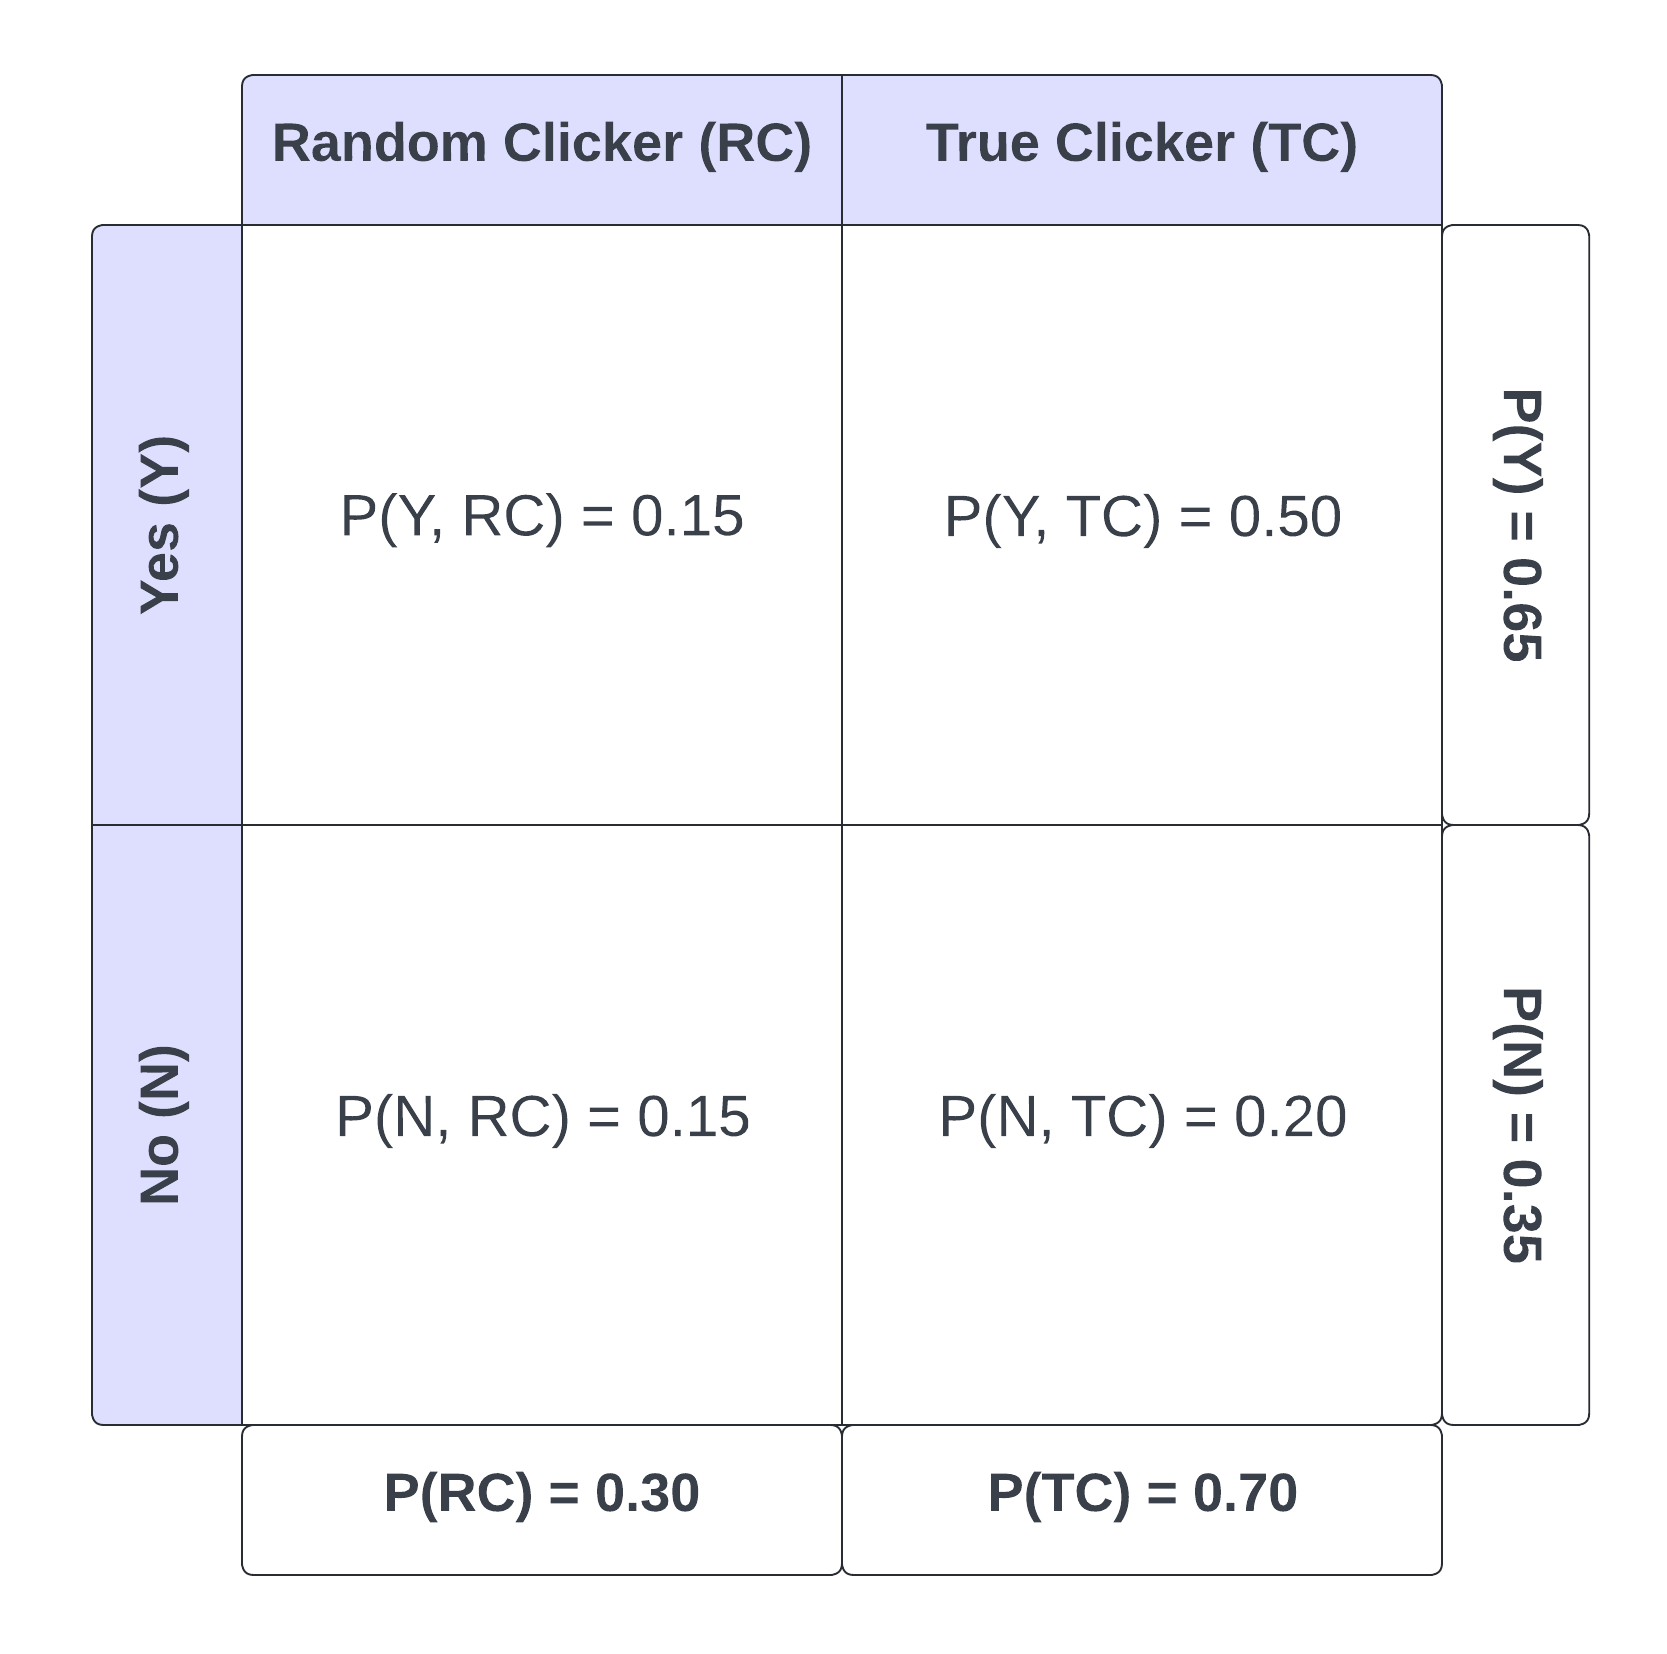
\includegraphics{Table.png}
\caption{alt}
\end{figure}

We're looking for P(Y\textbar TC) so we can use the rule of total
probability:

P(Y) = P(Y, TC) + P(Y, RC) = P(TC) * P(Y\textbar TC) + P(RC) *
P(Y\textbar RC)

We know all of these inputs to the equation except for P(Y\textbar TC),
so we want to solve for that unknown.

0.65 = 0.7 * P(Y\textbar TC) + 0.3 * 0.5

From the above equation, we find that P(Y\textbar TC) \(\approx\)
0.714286. This means that truthful clickers answer yes to the question
about 71.43\% of the time.

\hypertarget{part-b.}{%
\subsubsection{Part b.}\label{part-b.}}

P(Disease) = 0.000025 P(No Disease) = 0.999975 (1-0.000025)
P(Positive\textbar Disease) = .993 P(Negative\textbar No Disease) =
0.9999

The probabilities above are summarized in the tree diagram below:

\begin{figure}
\centering
\includegraphics{tree.png}
\caption{alt}
\end{figure}

We're looking for P(Disease\textbar Positive) so we can use Baye's Law:

\(\frac{P(Disease)*P(Positive|Disease)}{P(Disease)*P(Positive|Disease)+P(No Disease)*P(Positive|No Disease)}\)

We have almost all of the inputs that we need, however, we're missing
P(Positive\textbar No Disease). These are false positives. We can find
the missing probability by taking 1 - true negatives, or 1 - 0.9999 to
get P(Positive\textbar No Disease) as 0.0001. Now we can solve for
P(Disease\textbar Positive).

\(\frac{0.000025*0.993}{0.000025*0.993+0.999975*0.0001}\) \(\approx\)
.198882. Thus, if someone tests positive, they have about a 19.89\%
chance of actually having the disease.

\hypertarget{wrangling-the-billboard-top-100}{%
\section{Wrangling the Billboard Top
100}\label{wrangling-the-billboard-top-100}}

\begin{Shaded}
\begin{Highlighting}[]
\NormalTok{billboard }\OtherTok{=} \FunctionTok{read.csv}\NormalTok{(}\StringTok{"data/billboard.csv"}\NormalTok{)}
\end{Highlighting}
\end{Shaded}

\#Need a caption - probably something about how most are recent songs

\hypertarget{part-a.-1}{%
\subsubsection{Part a.}\label{part-a.-1}}

The table below shows the top 10 longest lasting songs on the Billboard
100. It reveals that a majority of these long-lasting songs are more
recent songs.

\hypertarget{part-b.-1}{%
\subsubsection{Part b.}\label{part-b.-1}}

\begin{Shaded}
\begin{Highlighting}[]
\NormalTok{musical\_diversity }\OtherTok{=}\NormalTok{ billboard }\SpecialCharTok{\%\textgreater{}\%}
  \FunctionTok{filter}\NormalTok{(year }\SpecialCharTok{!=} \DecValTok{1958} \SpecialCharTok{\&}\NormalTok{ year }\SpecialCharTok{!=} \DecValTok{2021}\NormalTok{) }\SpecialCharTok{\%\textgreater{}\%}
  \FunctionTok{group\_by}\NormalTok{(year) }\SpecialCharTok{\%\textgreater{}\%}
  \FunctionTok{summarize}\NormalTok{(}\AttributeTok{unique\_songs\_per\_year =} \FunctionTok{length}\NormalTok{(}\FunctionTok{unique}\NormalTok{(}\FunctionTok{c}\NormalTok{(performer,song))))}

\FunctionTok{ggplot}\NormalTok{(musical\_diversity) }\SpecialCharTok{+} \FunctionTok{geom\_line}\NormalTok{(}\FunctionTok{aes}\NormalTok{(}\AttributeTok{x =}\NormalTok{ year, }\AttributeTok{y =}\NormalTok{ unique\_songs\_per\_year)) }\SpecialCharTok{+} \FunctionTok{xlab}\NormalTok{(}\StringTok{"Year"}\NormalTok{) }\SpecialCharTok{+} \FunctionTok{ylab}\NormalTok{(}\StringTok{"Number of Unique Songs"}\NormalTok{) }\SpecialCharTok{+} \FunctionTok{ggtitle}\NormalTok{(}\StringTok{"Number of Unique Songs per Year"}\NormalTok{) }\SpecialCharTok{+} \FunctionTok{labs}\NormalTok{(}\AttributeTok{caption =} \StringTok{"As seen in the plot, the number of unique songs steadily decreased from roughly 1965 to a overall minimum of just below 700 songs around 2000. Since then, the trend has been increasing and in the last year of data (2020), there were about 1250 unique songs."}\NormalTok{)}
\end{Highlighting}
\end{Shaded}

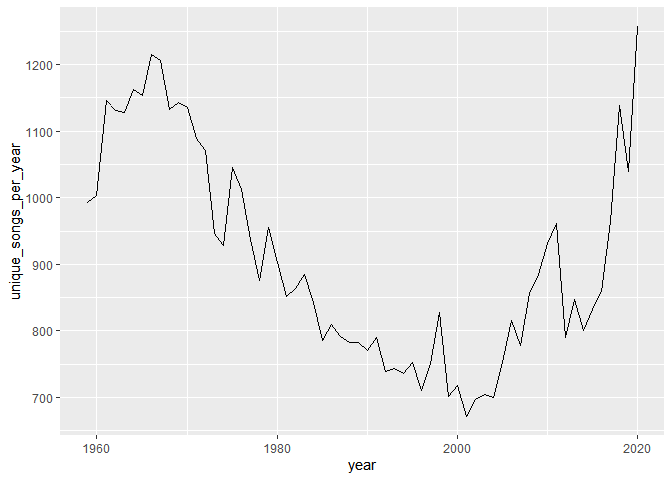
\includegraphics{STA-380-Part-2-Exercises_files/figure-latex/unnamed-chunk-4-1.pdf}

\hypertarget{part-c.}{%
\subsubsection{Part c.}\label{part-c.}}

\begin{Shaded}
\begin{Highlighting}[]
\NormalTok{ten\_week\_hit\_songs }\OtherTok{\textless{}{-}}\NormalTok{ billboard }\SpecialCharTok{\%\textgreater{}\%}
  \FunctionTok{group\_by}\NormalTok{(performer,song) }\SpecialCharTok{\%\textgreater{}\%}
  \FunctionTok{summarize}\NormalTok{(}\AttributeTok{ten\_week\_hit =} \FunctionTok{ifelse}\NormalTok{(}\FunctionTok{n}\NormalTok{()}\SpecialCharTok{\textgreater{}=}\DecValTok{10}\NormalTok{,}\StringTok{"Yes"}\NormalTok{,}\StringTok{"No"}\NormalTok{)) }\SpecialCharTok{\%\textgreater{}\%}
  \FunctionTok{filter}\NormalTok{(ten\_week\_hit }\SpecialCharTok{==} \StringTok{"Yes"}\NormalTok{)}
\end{Highlighting}
\end{Shaded}

\begin{verbatim}
## `summarise()` has grouped output by 'performer'. You can override using the
## `.groups` argument.
\end{verbatim}

\begin{Shaded}
\begin{Highlighting}[]
\NormalTok{top\_artists }\OtherTok{\textless{}{-}}\NormalTok{ ten\_week\_hit\_songs }\SpecialCharTok{\%\textgreater{}\%}
  \FunctionTok{group\_by}\NormalTok{(performer) }\SpecialCharTok{\%\textgreater{}\%}
  \FunctionTok{summarize}\NormalTok{(}\AttributeTok{num\_ten\_week\_hit =} \FunctionTok{n}\NormalTok{()) }\SpecialCharTok{\%\textgreater{}\%}
  \FunctionTok{filter}\NormalTok{(num\_ten\_week\_hit}\SpecialCharTok{\textgreater{}=}\DecValTok{30}\NormalTok{)}

\FunctionTok{ggplot}\NormalTok{(top\_artists) }\SpecialCharTok{+} \FunctionTok{geom\_bar}\NormalTok{(}\FunctionTok{aes}\NormalTok{(}\AttributeTok{x =} \FunctionTok{fct\_reorder}\NormalTok{(performer,num\_ten\_week\_hit), }\AttributeTok{y =}\NormalTok{ num\_ten\_week\_hit),}\AttributeTok{stat =} \StringTok{"identity"}\NormalTok{) }\SpecialCharTok{+} \FunctionTok{coord\_flip}\NormalTok{()}
\end{Highlighting}
\end{Shaded}

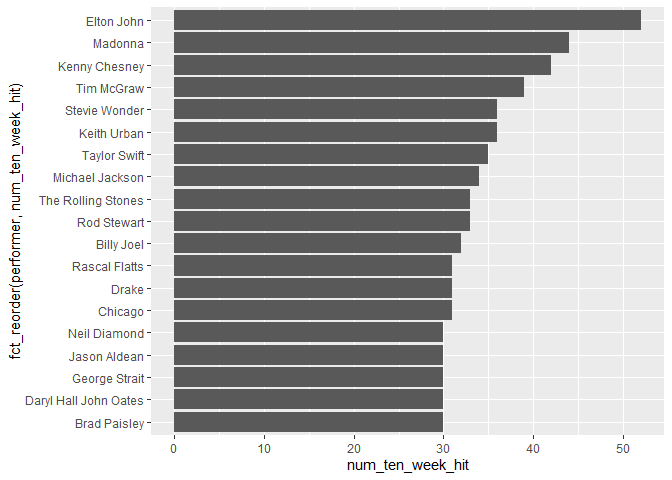
\includegraphics{STA-380-Part-2-Exercises_files/figure-latex/unnamed-chunk-5-1.pdf}

\#Visual story telling part 1: green buildings

\begin{Shaded}
\begin{Highlighting}[]
\NormalTok{green\_buildings }\OtherTok{=} \FunctionTok{read.csv}\NormalTok{(}\StringTok{"data/greenbuildings.csv"}\NormalTok{)}
\end{Highlighting}
\end{Shaded}

\begin{Shaded}
\begin{Highlighting}[]
\FunctionTok{ggplot}\NormalTok{(green\_buildings, }\FunctionTok{aes}\NormalTok{(}\AttributeTok{x =}\NormalTok{ Rent)) }\SpecialCharTok{+} \FunctionTok{geom\_histogram}\NormalTok{() }\SpecialCharTok{+} \FunctionTok{facet\_grid}\NormalTok{(.}\SpecialCharTok{\textasciitilde{}}\NormalTok{green\_rating)}
\end{Highlighting}
\end{Shaded}

\begin{verbatim}
## `stat_bin()` using `bins = 30`. Pick better value with `binwidth`.
\end{verbatim}

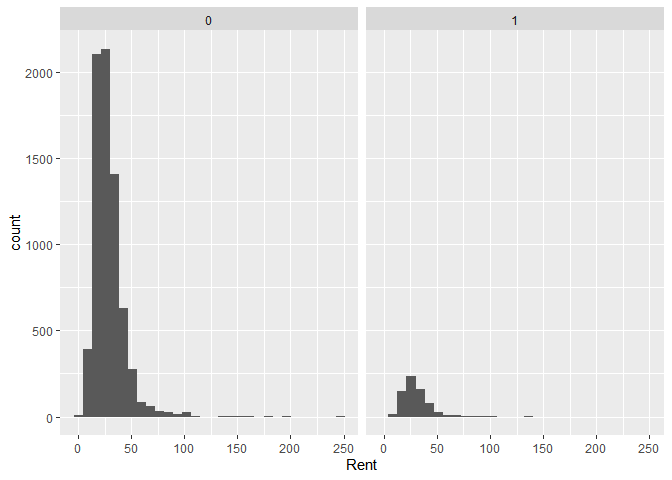
\includegraphics{STA-380-Part-2-Exercises_files/figure-latex/unnamed-chunk-7-1.pdf}

Green buildings tend to be newer, ``newness'' could justify higher rents

\begin{Shaded}
\begin{Highlighting}[]
\FunctionTok{ggplot}\NormalTok{(green\_buildings, }\FunctionTok{aes}\NormalTok{(}\AttributeTok{x =}\NormalTok{ green\_rating, }\AttributeTok{y =}\NormalTok{ age ,}\AttributeTok{group =}\NormalTok{ green\_rating)) }\SpecialCharTok{+} \FunctionTok{geom\_boxplot}\NormalTok{()}
\end{Highlighting}
\end{Shaded}

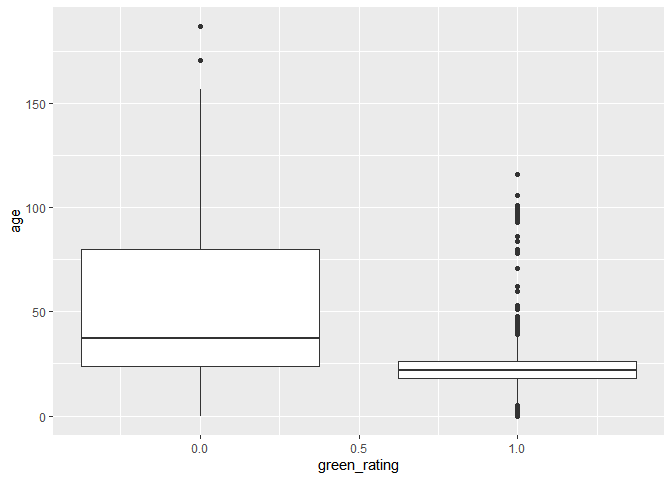
\includegraphics{STA-380-Part-2-Exercises_files/figure-latex/unnamed-chunk-8-1.pdf}

\begin{Shaded}
\begin{Highlighting}[]
\FunctionTok{ggplot}\NormalTok{(green\_buildings, }\FunctionTok{aes}\NormalTok{(}\AttributeTok{x =}\NormalTok{ age, }\AttributeTok{y =}\NormalTok{ Rent)) }\SpecialCharTok{+} \FunctionTok{geom\_line}\NormalTok{() }\SpecialCharTok{+} \FunctionTok{facet\_grid}\NormalTok{(. }\SpecialCharTok{\textasciitilde{}}\NormalTok{ green\_rating)}
\end{Highlighting}
\end{Shaded}

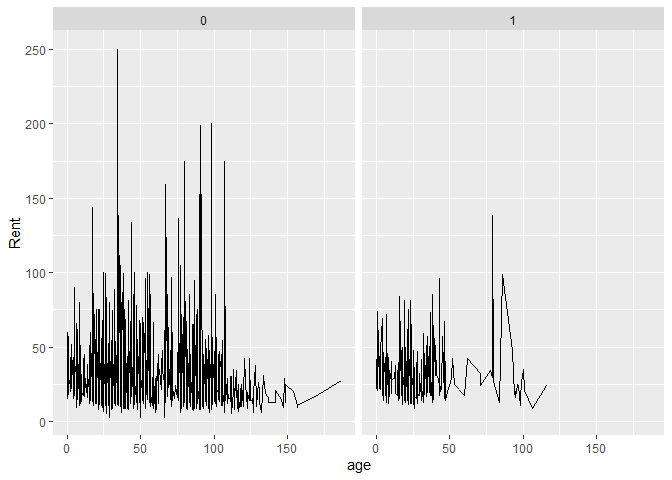
\includegraphics{STA-380-Part-2-Exercises_files/figure-latex/unnamed-chunk-9-1.pdf}

\hypertarget{visual-story-telling-part-2-cap-metro-data}{%
\section{Visual story telling part 2: Cap Metro
data}\label{visual-story-telling-part-2-cap-metro-data}}

\begin{Shaded}
\begin{Highlighting}[]
\NormalTok{cap\_metro }\OtherTok{\textless{}{-}} \FunctionTok{read.csv}\NormalTok{(}\StringTok{"data/capmetro\_UT.csv"}\NormalTok{)}
\end{Highlighting}
\end{Shaded}

\begin{Shaded}
\begin{Highlighting}[]
\NormalTok{cap\_metro}\SpecialCharTok{$}\NormalTok{time\_of\_day }\OtherTok{=} \FunctionTok{ifelse}\NormalTok{(cap\_metro}\SpecialCharTok{$}\NormalTok{hour\_of\_day }\SpecialCharTok{\%in\%} \FunctionTok{c}\NormalTok{(}\DecValTok{6}\NormalTok{,}\DecValTok{7}\NormalTok{,}\DecValTok{8}\NormalTok{,}\DecValTok{9}\NormalTok{,}\DecValTok{10}\NormalTok{,}\DecValTok{11}\NormalTok{),}\StringTok{"Morning"}\NormalTok{,}\FunctionTok{ifelse}\NormalTok{(cap\_metro}\SpecialCharTok{$}\NormalTok{hour\_of\_day }\SpecialCharTok{\%in\%} \FunctionTok{c}\NormalTok{(}\DecValTok{12}\NormalTok{,}\DecValTok{13}\NormalTok{,}\DecValTok{14}\NormalTok{,}\DecValTok{15}\NormalTok{,}\DecValTok{16}\NormalTok{),}\StringTok{"Afternoon"}\NormalTok{,}\StringTok{"Evening"}\NormalTok{))}
\NormalTok{time\_of\_day\_order }\OtherTok{\textless{}{-}} \FunctionTok{c}\NormalTok{(}\StringTok{"Morning"}\NormalTok{,}\StringTok{"Afternoon"}\NormalTok{,}\StringTok{"Evening"}\NormalTok{)}
\NormalTok{cap\_metro}\SpecialCharTok{$}\NormalTok{activity }\OtherTok{=}\NormalTok{ cap\_metro}\SpecialCharTok{$}\NormalTok{boarding }\SpecialCharTok{+}\NormalTok{ cap\_metro}\SpecialCharTok{$}\NormalTok{alighting}
\FunctionTok{ggplot}\NormalTok{(cap\_metro, }\FunctionTok{aes}\NormalTok{(}\AttributeTok{x =} \FunctionTok{factor}\NormalTok{(time\_of\_day,}\AttributeTok{levels=}\NormalTok{time\_of\_day\_order), }\AttributeTok{y =}\NormalTok{ activity)) }\SpecialCharTok{+} \FunctionTok{geom\_bar}\NormalTok{(}\AttributeTok{stat=}\StringTok{"identity"}\NormalTok{) }\SpecialCharTok{+} \FunctionTok{facet\_grid}\NormalTok{(. }\SpecialCharTok{\textasciitilde{}}\NormalTok{ weekend)}
\end{Highlighting}
\end{Shaded}

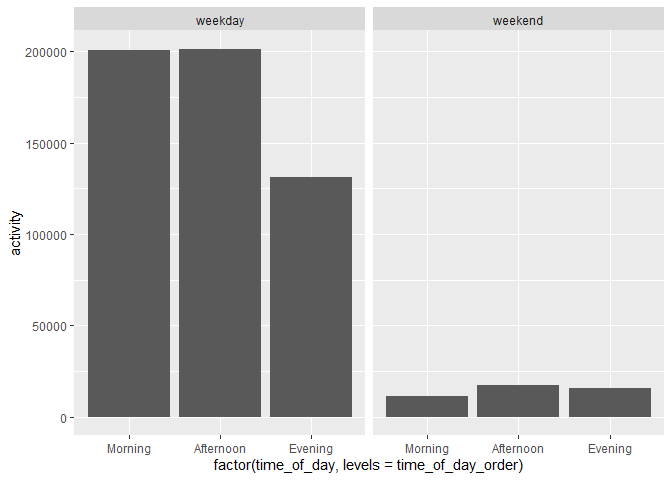
\includegraphics{STA-380-Part-2-Exercises_files/figure-latex/unnamed-chunk-11-1.pdf}

Activity seems to slightly increase as temperature increases, adjusted
for the difference in ridership between weekdays and weekends

\begin{Shaded}
\begin{Highlighting}[]
\NormalTok{riders\_temp }\OtherTok{=}\NormalTok{ cap\_metro }\SpecialCharTok{\%\textgreater{}\%}
  \FunctionTok{group\_by}\NormalTok{(timestamp) }\SpecialCharTok{\%\textgreater{}\%}
  \FunctionTok{summarize}\NormalTok{(}\AttributeTok{total\_riders =} \FunctionTok{sum}\NormalTok{(activity), }\AttributeTok{mean\_temp =} \FunctionTok{mean}\NormalTok{(temperature), }\AttributeTok{weekend =}\NormalTok{ weekend)}
\FunctionTok{ggplot}\NormalTok{(riders\_temp, }\FunctionTok{aes}\NormalTok{(}\AttributeTok{x =}\NormalTok{ mean\_temp, }\AttributeTok{y =}\NormalTok{ total\_riders)) }\SpecialCharTok{+} \FunctionTok{geom\_line}\NormalTok{()}\SpecialCharTok{+}\FunctionTok{facet\_grid}\NormalTok{(.}\SpecialCharTok{\textasciitilde{}}\NormalTok{weekend)}
\end{Highlighting}
\end{Shaded}

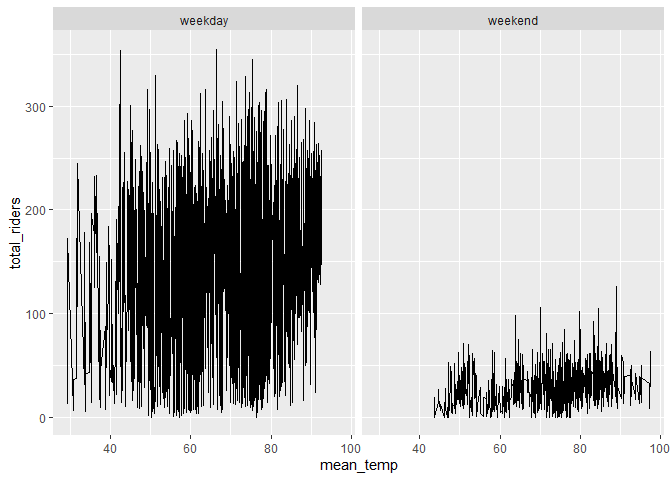
\includegraphics{STA-380-Part-2-Exercises_files/figure-latex/unnamed-chunk-12-1.pdf}

\hypertarget{clustering-and-pca}{%
\section{Clustering and PCA}\label{clustering-and-pca}}

\begin{Shaded}
\begin{Highlighting}[]
\NormalTok{wine }\OtherTok{\textless{}{-}} \FunctionTok{read.csv}\NormalTok{(}\StringTok{"data/wine.csv"}\NormalTok{)}
\end{Highlighting}
\end{Shaded}

\begin{Shaded}
\begin{Highlighting}[]
\FunctionTok{set.seed}\NormalTok{(}\DecValTok{1}\NormalTok{)}
\NormalTok{wine\_quant }\OtherTok{\textless{}{-}}\NormalTok{ wine[,}\SpecialCharTok{!} \FunctionTok{names}\NormalTok{(wine) }\SpecialCharTok{\%in\%} \FunctionTok{c}\NormalTok{(}\StringTok{"color"}\NormalTok{,}\StringTok{"quality"}\NormalTok{)]}
\NormalTok{wine\_pca }\OtherTok{=} \FunctionTok{prcomp}\NormalTok{(wine\_quant, }\AttributeTok{rank=}\DecValTok{10}\NormalTok{, }\AttributeTok{scale=}\ConstantTok{TRUE}\NormalTok{)}
\FunctionTok{boxplot}\NormalTok{(wine\_pca}\SpecialCharTok{$}\NormalTok{x[,}\DecValTok{1}\NormalTok{],}\FunctionTok{as.factor}\NormalTok{(wine}\SpecialCharTok{$}\NormalTok{color))}
\end{Highlighting}
\end{Shaded}

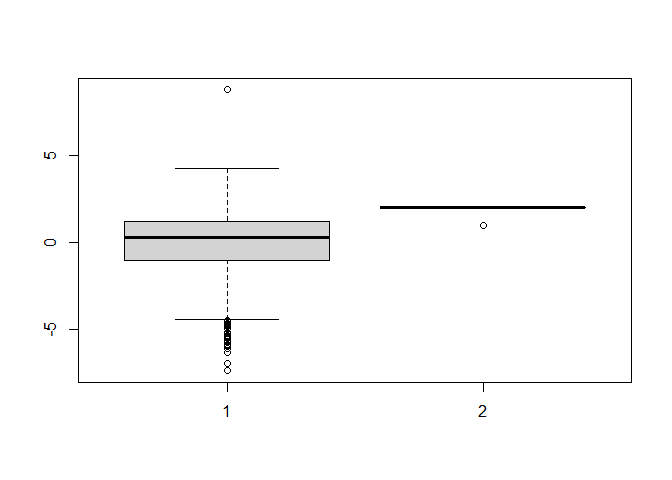
\includegraphics{STA-380-Part-2-Exercises_files/figure-latex/unnamed-chunk-14-1.pdf}

Cluster 1 is mostly red wines, whereas Cluster 2 is mostly white wines.
Even just making two clusters distinguishes between the two wine colors
very well.

\begin{Shaded}
\begin{Highlighting}[]
\FunctionTok{set.seed}\NormalTok{(}\DecValTok{1}\NormalTok{)}
\FunctionTok{library}\NormalTok{(knitr)}
\NormalTok{wine\_quant\_scaled }\OtherTok{\textless{}{-}} \FunctionTok{scale}\NormalTok{(wine\_quant)}
\NormalTok{wine\_clusters }\OtherTok{\textless{}{-}} \FunctionTok{kmeans}\NormalTok{(wine\_quant\_scaled, }\AttributeTok{centers=}\DecValTok{2}\NormalTok{, }\AttributeTok{nstart=}\DecValTok{50}\NormalTok{)}
\FunctionTok{table}\NormalTok{(wine\_clusters}\SpecialCharTok{$}\NormalTok{cluster,wine}\SpecialCharTok{$}\NormalTok{color)}
\end{Highlighting}
\end{Shaded}

\begin{verbatim}
##    
##      red white
##   1 1575    68
##   2   24  4830
\end{verbatim}

While the 2 clusters separated out the two wine colors well, they don't
seem to distinguish between wine quality because the median quality is
essentially the same for both clusters. Even if we increase the number
of clusters pretty dramatically up to 10, there still doesn't appear to
be major quality differences between the boxplots.

\begin{Shaded}
\begin{Highlighting}[]
\NormalTok{wine}\SpecialCharTok{$}\NormalTok{cluster }\OtherTok{=} \FunctionTok{as.factor}\NormalTok{(wine\_clusters}\SpecialCharTok{$}\NormalTok{cluster)}
\FunctionTok{ggplot}\NormalTok{(wine, }\FunctionTok{aes}\NormalTok{(}\AttributeTok{x =}\NormalTok{ cluster, }\AttributeTok{y =}\NormalTok{ quality)) }\SpecialCharTok{+} \FunctionTok{geom\_boxplot}\NormalTok{()}
\end{Highlighting}
\end{Shaded}

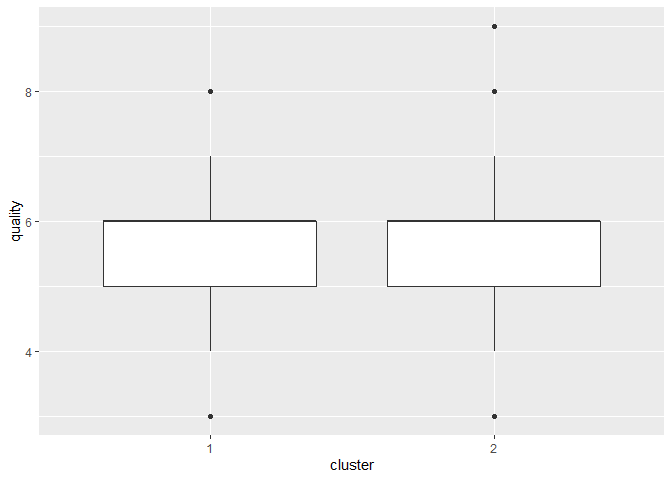
\includegraphics{STA-380-Part-2-Exercises_files/figure-latex/unnamed-chunk-16-1.pdf}

\textless\textless\textless\textless\textless\textless\textless{} HEAD

\hypertarget{market-segmentation}{%
\section{\#Market Segmentation}\label{market-segmentation}}

\hypertarget{market-segmentation-1}{%
\section{Market Segmentation}\label{market-segmentation-1}}

\begin{quote}
\begin{quote}
\begin{quote}
\begin{quote}
\begin{quote}
\begin{quote}
\begin{quote}
243a1b6b2111a88510e69fdd65cfde561c881fbc
\end{quote}
\end{quote}
\end{quote}
\end{quote}
\end{quote}
\end{quote}
\end{quote}

We decided to define market segments for this problem as clusters
identified through the k-means clustering approach. We omitted the
Twitter user's randomly generated ID when creating the clusters and
instead only used the scores for each Tweet interest. We settled on
creating 10 market segments (clusters) as 10 seemed to be a sweet spot
between capturing legitimate differences between Twitter followers while
also not overloading the company with too many market segments to try to
understand.

While NutrientH20 might be interested in all 10 of the market segments
that we've identified, they'll likely care the most about the segments
that would be most receptive to their products. Thus, we found the 3
market segments with the highest average scores for the
``health\_nutrition'' interest given that NutrientH20 seems to be a
health-oriented company. The summaries of the three segments are below:

\begin{verbatim}
##    Market Segment Interest Category Average Score
## 1               1  health_nutrition     12.541667
## 2               1  personal_fitness      6.651042
## 3               1           chatter      3.941406
## 4               1           cooking      3.425781
## 5               1          outdoors      2.876302
## 6               1     photo_sharing      2.399740
## 7               1              food      2.205729
## 8               1    current_events      1.514323
## 9               1          shopping      1.283854
## 10              1            travel      1.229167
## 11              3           cooking     11.684211
## 12              3     photo_sharing      6.088421
## 13              3           fashion      5.985263
## 14              3           chatter      4.246316
## 15              3            beauty      4.208421
## 16              3  health_nutrition      2.269474
## 17              3          shopping      1.755789
## 18              3    current_events      1.751579
## 19              3       college_uni      1.496842
## 20              3            travel      1.461053
## 21              4           chatter      4.653061
## 22              4  health_nutrition      2.795918
## 23              4     photo_sharing      2.448980
## 24              4            travel      2.244898
## 25              4          politics      2.244898
## 26              4       college_uni      1.918367
## 27              4     sports_fandom      1.897959
## 28              4    current_events      1.877551
## 29              4           cooking      1.795918
## 30              4  personal_fitness      1.755102
\end{verbatim}

From the three most promising market segments, the first one appears to
be the most appealing to NutrientH20. Members of this segment have by
far the highest average scores for the ``health\_nutrition'' interst
category, and also have high average scores for ``fitness'' which
probably is something closely related to what NutrientH20 does as well.
There are 768 Twitter users in the most promising market segment of
segment 1, and then 475 and 49 in segments 3 and 4, respectively.
Focusing in on these market segment will hopefully yield more future
customers than trying to market to all Twitter followers.

\hypertarget{head}{%
\section{\textless\textless\textless\textless\textless\textless\textless{}
HEAD}\label{head}}

\hypertarget{the-reuters-corpus}{%
\section{The Reuters Corpus}\label{the-reuters-corpus}}

\textbf{Figure out how to download this data} - For now, just clone the
Github and copy the folder over; I've added it to .gitignore so it won't
be pushed to Github

\begin{quote}
\begin{quote}
\begin{quote}
\begin{quote}
\begin{quote}
\begin{quote}
\begin{quote}
243a1b6b2111a88510e69fdd65cfde561c881fbc \# Association Rule Mining
\end{quote}
\end{quote}
\end{quote}
\end{quote}
\end{quote}
\end{quote}
\end{quote}

\begin{Shaded}
\begin{Highlighting}[]
\FunctionTok{library}\NormalTok{(arules)}
\end{Highlighting}
\end{Shaded}

\begin{verbatim}
## Warning: package 'arules' was built under R version 4.1.3
\end{verbatim}

\begin{verbatim}
## Loading required package: Matrix
\end{verbatim}

\begin{verbatim}
## 
## Attaching package: 'arules'
\end{verbatim}

\begin{verbatim}
## The following object is masked from 'package:dplyr':
## 
##     recode
\end{verbatim}

\begin{verbatim}
## The following objects are masked from 'package:base':
## 
##     abbreviate, write
\end{verbatim}

\begin{Shaded}
\begin{Highlighting}[]
\FunctionTok{library}\NormalTok{(reshape2)}
\CommentTok{\#Read in the groceries.txt file. Find max number of objects}
\CommentTok{\#in a basket so that R doesn\textquotesingle{}t automatically cap the number}
\CommentTok{\#of columns we can have}
\NormalTok{no\_col }\OtherTok{\textless{}{-}} \FunctionTok{max}\NormalTok{(}\FunctionTok{count.fields}\NormalTok{(}\StringTok{"groceries.txt"}\NormalTok{, }\AttributeTok{sep =} \StringTok{","}\NormalTok{))}
\NormalTok{groceries }\OtherTok{\textless{}{-}} \FunctionTok{read.table}\NormalTok{(}\StringTok{"groceries.txt"}\NormalTok{,}\AttributeTok{sep=}\StringTok{","}\NormalTok{,}\AttributeTok{fill=}\ConstantTok{TRUE}\NormalTok{,}\AttributeTok{col.names=}\FunctionTok{c}\NormalTok{(}\DecValTok{1}\SpecialCharTok{:}\NormalTok{no\_col))}
\NormalTok{no\_col }\OtherTok{\textless{}{-}} \FunctionTok{max}\NormalTok{(}\FunctionTok{count.fields}\NormalTok{(}\StringTok{"data/groceries.txt"}\NormalTok{, }\AttributeTok{sep =} \StringTok{","}\NormalTok{))}
\NormalTok{groceries }\OtherTok{\textless{}{-}} \FunctionTok{read.table}\NormalTok{(}\StringTok{"data/groceries.txt"}\NormalTok{,}\AttributeTok{sep=}\StringTok{","}\NormalTok{,}\AttributeTok{fill=}\ConstantTok{TRUE}\NormalTok{,}\AttributeTok{col.names=}\FunctionTok{c}\NormalTok{(}\DecValTok{1}\SpecialCharTok{:}\NormalTok{no\_col))}
\CommentTok{\#Add in a column that indicates which customer corresponds to }
\CommentTok{\#the basket (row number)}
\NormalTok{groceries}\SpecialCharTok{$}\NormalTok{customer }\OtherTok{=} \FunctionTok{as.factor}\NormalTok{(}\DecValTok{1}\SpecialCharTok{:}\FunctionTok{nrow}\NormalTok{(groceries))}
\CommentTok{\#Get data in long format}
\NormalTok{groceries }\OtherTok{\textless{}{-}} \FunctionTok{melt}\NormalTok{(groceries,}\AttributeTok{id.vars =} \StringTok{\textquotesingle{}customer\textquotesingle{}}\NormalTok{) }
\NormalTok{groceries }\OtherTok{\textless{}{-}} \FunctionTok{as.data.frame}\NormalTok{(groceries)}
\CommentTok{\#Drop all values that are blank}
\NormalTok{groceries }\OtherTok{\textless{}{-}} \FunctionTok{subset}\NormalTok{(groceries, groceries}\SpecialCharTok{$}\NormalTok{value }\SpecialCharTok{!=} \StringTok{""}\NormalTok{)}
\CommentTok{\#Group the grocery products by the customer who bought them}
\NormalTok{groceries }\OtherTok{\textless{}{-}} \FunctionTok{split}\NormalTok{(}\AttributeTok{x=}\NormalTok{groceries}\SpecialCharTok{$}\NormalTok{value, }\AttributeTok{f=}\NormalTok{groceries}\SpecialCharTok{$}\NormalTok{customer)}
\CommentTok{\#Make sure each customer is only associated with unique}
\CommentTok{\#products in their basket}
\NormalTok{groceries }\OtherTok{\textless{}{-}} \FunctionTok{lapply}\NormalTok{(groceries, unique)}
\end{Highlighting}
\end{Shaded}

\begin{Shaded}
\begin{Highlighting}[]
\FunctionTok{library}\NormalTok{(arulesViz)}
\end{Highlighting}
\end{Shaded}

\begin{verbatim}
## Warning: package 'arulesViz' was built under R version 4.1.3
\end{verbatim}

\begin{Shaded}
\begin{Highlighting}[]
\NormalTok{interesting\_rules }\OtherTok{\textless{}{-}} \FunctionTok{head}\NormalTok{(}\FunctionTok{sort}\NormalTok{(groceries\_rules, }\AttributeTok{by=}\StringTok{"lift"}\NormalTok{), }\DecValTok{10}\NormalTok{)}
\FunctionTok{plot}\NormalTok{(interesting\_rules, }\AttributeTok{method=}\StringTok{"grouped"}\NormalTok{)}
\end{Highlighting}
\end{Shaded}

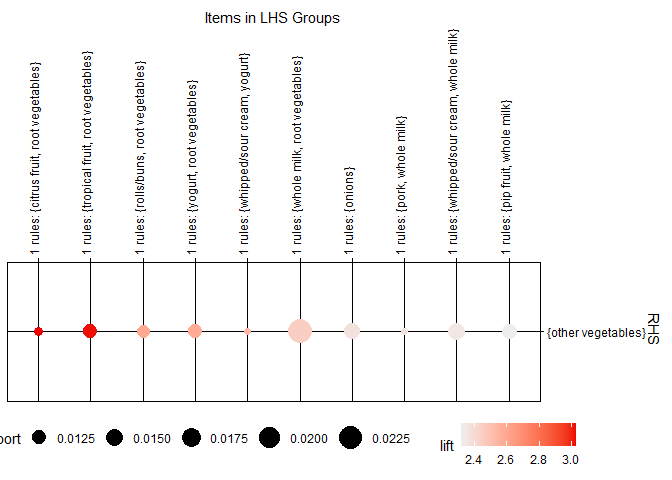
\includegraphics{STA-380-Part-2-Exercises_files/figure-latex/unnamed-chunk-22-1.pdf}

\begin{Shaded}
\begin{Highlighting}[]
\FunctionTok{itemFrequencyPlot}\NormalTok{(}\FunctionTok{items}\NormalTok{(groceries\_rules),}\AttributeTok{population=}\NormalTok{groceries\_trans,}\AttributeTok{topN=}\DecValTok{10}\NormalTok{,}\AttributeTok{popCol=}\StringTok{"red"}\NormalTok{)}
\end{Highlighting}
\end{Shaded}

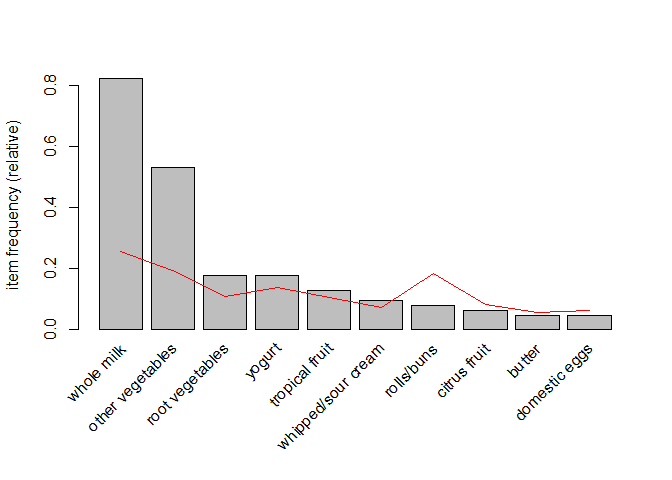
\includegraphics{STA-380-Part-2-Exercises_files/figure-latex/unnamed-chunk-23-1.pdf}

\begin{Shaded}
\begin{Highlighting}[]
\NormalTok{whole\_milk\_rules }\OtherTok{\textless{}{-}} \FunctionTok{apriori}\NormalTok{(groceries\_trans, }
    \AttributeTok{parameter=}\FunctionTok{list}\NormalTok{(}\AttributeTok{support=}\NormalTok{.}\DecValTok{01}\NormalTok{, }\AttributeTok{confidence=}\NormalTok{.}\DecValTok{4}\NormalTok{, }\AttributeTok{maxlen=}\DecValTok{4}\NormalTok{),}\AttributeTok{appearance =} \FunctionTok{list}\NormalTok{(}\AttributeTok{default=}\StringTok{"lhs"}\NormalTok{, }\AttributeTok{rhs=}\StringTok{"whole milk"}\NormalTok{))}
\end{Highlighting}
\end{Shaded}

\begin{verbatim}
## Apriori
## 
## Parameter specification:
##  confidence minval smax arem  aval originalSupport maxtime support minlen
##         0.4    0.1    1 none FALSE            TRUE       5    0.01      1
##  maxlen target  ext
##       4  rules TRUE
## 
## Algorithmic control:
##  filter tree heap memopt load sort verbose
##     0.1 TRUE TRUE  FALSE TRUE    2    TRUE
## 
## Absolute minimum support count: 98 
## 
## set item appearances ...[1 item(s)] done [0.00s].
## set transactions ...[169 item(s), 9835 transaction(s)] done [0.00s].
## sorting and recoding items ... [88 item(s)] done [0.00s].
## creating transaction tree ... done [0.00s].
## checking subsets of size 1 2 3 4
\end{verbatim}

\begin{verbatim}
## Warning in apriori(groceries_trans, parameter = list(support = 0.01, confidence
## = 0.4, : Mining stopped (maxlen reached). Only patterns up to a length of 4
## returned!
\end{verbatim}

\begin{verbatim}
##  done [0.00s].
## writing ... [43 rule(s)] done [0.00s].
## creating S4 object  ... done [0.00s].
\end{verbatim}

\begin{Shaded}
\begin{Highlighting}[]
\FunctionTok{length}\NormalTok{(whole\_milk\_rules)}\SpecialCharTok{/}\FunctionTok{length}\NormalTok{(groceries\_rules)}
\end{Highlighting}
\end{Shaded}

\begin{verbatim}
## [1] 0.6935484
\end{verbatim}

\begin{Shaded}
\begin{Highlighting}[]
\CommentTok{\#Export to a graphml file so that we can visualize this data in Gephi}
\FunctionTok{library}\NormalTok{(igraph)}
\end{Highlighting}
\end{Shaded}

\begin{verbatim}
## Warning: package 'igraph' was built under R version 4.1.2
\end{verbatim}

\begin{verbatim}
## 
## Attaching package: 'igraph'
\end{verbatim}

\begin{verbatim}
## The following object is masked from 'package:arules':
## 
##     union
\end{verbatim}

\begin{verbatim}
## The following objects are masked from 'package:dplyr':
## 
##     as_data_frame, groups, union
\end{verbatim}

\begin{verbatim}
## The following objects are masked from 'package:stats':
## 
##     decompose, spectrum
\end{verbatim}

\begin{verbatim}
## The following object is masked from 'package:base':
## 
##     union
\end{verbatim}

\begin{Shaded}
\begin{Highlighting}[]
\NormalTok{groceries\_graph }\OtherTok{=} \FunctionTok{associations2igraph}\NormalTok{(}\FunctionTok{subset}\NormalTok{(groceries\_rules, lift}\SpecialCharTok{\textgreater{}}\DecValTok{1}\NormalTok{), }\AttributeTok{associationsAsNodes =} \ConstantTok{FALSE}\NormalTok{)}
\NormalTok{igraph}\SpecialCharTok{::}\FunctionTok{write\_graph}\NormalTok{(groceries\_graph, }\AttributeTok{file=}\StringTok{\textquotesingle{}groceries.graphml\textquotesingle{}}\NormalTok{, }\AttributeTok{format =} \StringTok{"graphml"}\NormalTok{)}
\end{Highlighting}
\end{Shaded}

======= \#Export to a graphml file so that we can visualize this data in
Gephi library(igraph) library(arulesViz) groceries\_graph =
associations2igraph(subset(groceries\_rules, lift\textgreater1),
associationsAsNodes = FALSE) igraph::write\_graph(groceries\_graph,
file=`groceries.graphml', format = ``graphml'') ```
\textgreater\textgreater\textgreater\textgreater\textgreater\textgreater\textgreater{}
243a1b6b2111a88510e69fdd65cfde561c881fbc

\end{document}
